\documentclass[a4paper, 12pt]{book}

\usepackage[T1]{fontenc}
\usepackage[utf8]{inputenc}
\usepackage[italian]{babel}
\usepackage[colorlinks]{hyperref}
\usepackage{listings}
\usepackage{xcolor}
\usepackage{graphicx}

\definecolor{codegreen}{rgb}{0,0.6,0}
\definecolor{codegray}{rgb}{0.5,0.5,0.5}
\definecolor{codepurple}{rgb}{0.58,0,0.82}
\definecolor{backcolour}{rgb}{0.95,0.95,0.92}

\lstdefinestyle{mystyle}{
    backgroundcolor=\color{backcolour},   
    commentstyle=\color{codegreen},
    keywordstyle=\color{violet},
    numberstyle=\tiny\color{codegray},
    stringstyle=\color{codepurple},
    basicstyle=\ttfamily\footnotesize,
    breakatwhitespace=false,         
    breaklines=true,                 
    captionpos=b,                    
    keepspaces=true,                 
    numbers=left,                    
    numbersep=5pt,                  
    showspaces=false,                
    showstringspaces=false,
    showtabs=false,                  
    tabsize=2
}

\lstset{style=mystyle}

\title{Laboratorio Sistemi Operativi}
\author{Giovanni Tosini}
\date{}

\begin{document}

    \begin{titlepage}
        \maketitle
    \end{titlepage}

    \frontmatter
    \tableofcontents
    \mainmatter

    \chapter{Processi e programmi}

    Un processo è un'istanza di un programma eseguito.
    Come viene creato, il \textbf{Kernel} gli associa
    una certa struttura di memoria.
    \begin{description}
        \item[Program code:] segmento in sola lettura  contenente istruzioni in linguaggio macchina;
        \item[Initialized data:] segmento contenente variabili globali e statiche;
        \item[Uninitialized data:] segmente contenente variabili globali e statiche \textbf{non} inizializzate;
        \item[Heap:] segmento contenente variabili allocate dinamicamente;
        \item[Stack:] segmento contenente gli argomenti e le variabili interne delle funzioni.    
    \end{description}
    Una delle strutture dati di supporto è il \textbf{file
    descriptor table}, conterrà tutti i file che il 
    processo aprirà. Ogni processo contiene già 3 
    \textbf{file descriptor} associati ad esso:
    \begin{enumerate}
        \item Standard input
        \item Standard output
        \item Standard error
    \end{enumerate}
    Ogni successivo file aperto verrà identificato con 
    il valore minore disponibile. Il file descriptor
    table è visibile \textbf{solo} a runtime.

    \chapter{System call}

    Sono un punto di ingresso verso il Kernel, vengono 
    utilizzate per richiedere dei servizi. Dallo User Level 
    verranno fatte delle chiamate alla System Call 
    Interface che a sua volta comunicherà al Kernel.

    \section{Gestione degli errori delle System Call}

    Nella sezione ERRORS del comando \verb|man| si possono trovare
    tutti i possibili valori di ritorno di errore di una 
    System Call. Tuttavia è possibile usare la variabile 
    \verb|errno| accedibile tramite l'uso della libreria
    \verb|<errno.h>|. Ci permetterà di sapere l'errore 
    effettivo causato in base al valore salvato al suo 
    interno.

    Esempio:
    \begin{lstlisting}[language=C]
        #include <errno.h>
        ...
        //system call to open a file
        fd = open(pathname, flags, mode);
        //Begin code handling errors
        if(fd == -1){
            if(errno == EACCES){
                //Handling not allowed access to the file
            }
            else{
                //Some other error occured
            }
        }
        //End code handling errors
        ...
    \end{lstlisting}
    La maggior parte delle system call ritorna un -1 
    o NULL Pointer in caso di errore, alcune però 
    usano il -1 come valore di ritorno anche in caso di 
    non errore. Qui l'uso di \verb|errno| acquista 
    ulteriore valore. Esempio:
    \begin{lstlisting}[language=C]
        #include <sys/resource.h>
        ... 
        //Reset the errno variable to 0
        errno = 0;
        //System call getpriority gets the nice value of a process 
        nice = getpriority(which, who);
        if((nice == -1) && (errno != 0)){
            //Handling getpriority errors
        }
        ...        
    \end{lstlisting}
    
    Esistono altre funzioni che aiutano a gestire gli 
    errori, come la funzione \verb|perror()| che stampa 
    su standard error la stringa che le viene fornita.
    Esempio:
    \begin{lstlisting}[language=C]
        #include <stdio.h>
        ... 
        //System call to open a file
        fd = open(pathname, flags, mode);
        if(fd == -1){
            perror("<Open>");
            //System call to kill the current process
            exit(EXIT_FAILURE);
        }
        ...
    \end{lstlisting}
    L'output sarà:
    \begin{lstlisting}[language=C]
        <Open>: No such file or directory
    \end{lstlisting}
    
    La libreria \verb|string.h| fornisce la funzione 
    \verb|strerror()| che prende in input il valore di 
    \verb|errno| e stampa l'errore effettivo. Esempio:
    \begin{lstlisting}[language=C]
        #include <stdio.h>
        ... 
        //System call to open a file
        fd = open(path, flags, mode);
        if(fd == -1){
            printf("Error opening (%s): \n\t%s\n", path, strerror(errno));
            //System call to kill the current process
            exit(EXIT_FAILURE);
        }
        ...
    \end{lstlisting}
    L'output sarà il seguente:
    \begin{lstlisting}[language=C]
        Error opening (myFile.txt):
            No such file or directory        
    \end{lstlisting}

    \chapter{Kernel data types}

    Sono delle \verb|typedef| di tipi normali C, necessari
    per ovviare problemi di portabilità, per esempio 
    il \verb|pid_t| usando per identificare il process ID
    di un processo non è altro che un tipo definito come 
    \verb|typedef int pid_t|, quindi un intero.
    
    \chapter{Filesystem}

    \section{File}

    \subsection{open}

    Apre un file esistente e nel caso in cui non esistesse 
    lo può creare tramite l'uso di specifiche flag, in caso di 
    successo ritorna un file descriptor, quindi va aggiunta 
    una riga alla file descriptor table. In caso di errore
    ritorna un -1.
    \begin{lstlisting}[language=C]
        #include <sys/stat.h>
        #include <stdio.h>

        //Returns file descriptor on successo, or -1 on error 
        int open(const char *pathname, int flags, .../*mode_t mode*/);
    \end{lstlisting}
    \begin{itemize}
        \item il \verb|pathname| può essere il nome del file o il suo eventuale path;
        \item la flag può essere un bit mask di una o più flag che definiscono l'accesso al file, possono essere ORate fra di loro tramite "|";
        \item le mode possono si comportano in maniera simile alle flag, definiscono i permessi che il file avrà.
    \end{itemize}
    Tabella con le flag disponibili:
    \begin{center}
        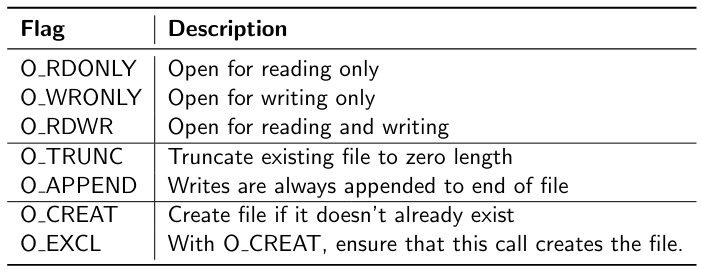
\includegraphics[width=0.5\textwidth]{flag_open.png}
    \end{center}
    Tabella delle mode disponibili:
    \begin{center}
        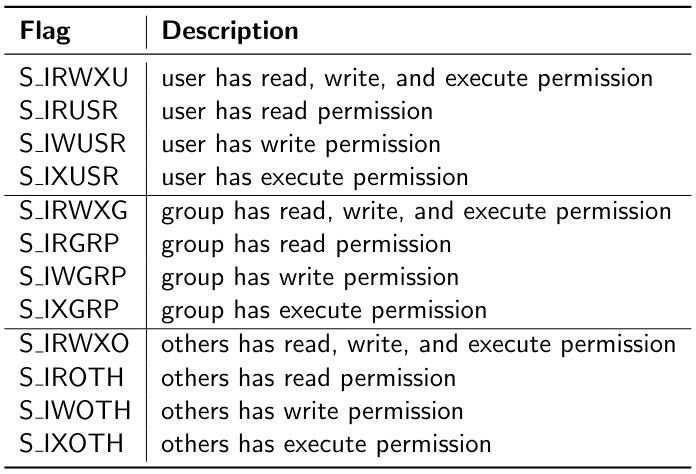
\includegraphics[width=0.5\textwidth]{mode_open.png}
    \end{center}
    Se non vengono forniti i permessi cosa succederà al file?
    All'interno del SO esiste la \verb|umask| con dei valori che 
    di default non dà permessi allo user e solo scrittura
    a group e others, tale valore sarà 022. Di \verb|umask|
    ne esiste una sola, andando a fornire dei permessi tramite 
    la \verb|open| i permessi che il file avrà saranno 
    la \verb|mode| con il negato della \verb|umask| (mode and
    $\sim$umask. 
    Vari esempi di utilizzo:
    \begin{lstlisting}[language=C]
        int fd;
        //Open existing file for only writing
        fd = open("myfile", O_WRONLY);

        //Open new or existing file for reading/writing, truncating 
        // to zero bytes; file permissions read+write only for owner
        fd = open("myfile", O_RDWR | O_CREAT | O_TRUNC, S_IRUSR | S_IWUSR);
    \end{lstlisting}
    
    \subsection{read}

    Prende in input il file descriptor ottenuto tramite la 
     \verb|open|, un \verb|buffer| dove andremo a salvare quello che 
    leggeremo dal file e un \verb|size_t| che definisce il numero di byte 
    che vogliamo leggere dal file. In caso di successo ritornerà 
    un valore \verb|ssize_t| che dovrebbe essere uguale o minore a \verb|count|, in di
    errore tornerà un -1.
    \begin{lstlisting}[language=C]
        #include <stdio.h> 

        //Returns number of bytes read, or -1 on error
        ssize_t read(int fd, void *buf, size_t count);
    \end{lstlisting}
    Esempio d'uso:
    \begin{lstlisting}[language=C]
        //Open existing file for reading
        int fd = open("myfile", O_RDONLY);
        if(fd == -1)
            errExit("open");
        
        // A MAX_READ bytes buffer
        char buffer[MAX_READ + 1];

        //Reading up to MAX_READ bytes from myfile
        ssize_t numRead = read(fd, buffer, MAX_READ);
        if(numRead == -1)
            errExit("Read");
    \end{lstlisting}
    Un esempio di lettura da Standard Input:
    \begin{lstlisting}[language=C]
        // A MAX_READ bytes buffer
        char buffer[MAX_READ + 1];

        //Reading up to MAX_READ bytes from STDIN
        ssize_t numRead = read(STDIN_FILENO, buffer, MAX_READ);
        if(numRead == -1)
            errExit("read");
        
        buffer[numRead] = '\0';
        printf("Input data: %s\n", buffer);
    \end{lstlisting}

    \subsection{write}

    Ci permette di scrivere su un file descriptor
    \begin{lstlisting}[language=C]
        #include <unistd.h>

        //Returns number of bytes written, or -1 on error
        sszie_t write(int fd, void *buf, size_t count);
    \end{lstlisting}
    Esempio di scrittura:
    \begin{lstlisting}[language=C]
        //Open existing file fro writing
        int fd = open("myfile", O_WRONLY);
        int(fd == -1)
            errExit("open");

        //A buffer collecting the string
        char buffer[] = "Ciao Mondo";

        //Writing up to sizeof(buffer) bytes into myfile
        ssize_t numWrite = write(fd, buffer, sizeof(buffer));
        if(numWrite != sizeof(buffer))
            errExit("write");
    \end{lstlisting}
    Per scrivere su terminale, come prima si userà \verb|STDOUT_FILENO| al posto del file descriptor.

    \subsection{lseek}

    Una volta aperto un file, il kernel salva un file offset
    ovvero un indicatore un valore che identifica a quale punto 
    di scrittura/lettura siamo arrivati. Per utilizzare tale 
    cursore useremo la \verb|lseek|.
    \begin{lstlisting}[language=C]
        #include <unistd.h>

        //Returns the resulting offset location, or -1 on error
        off_t write(int fd, off_t offset, int whence);
    \end{lstlisting}
    \begin{description}
        \item[N.B.:] \verb|whence| indica la base di partenza dell'offset; 
    \end{description}
    Esempio di utilizzo:
    \begin{lstlisting}[language=C]
        #include <unistd.h>

        //Returns number of bytes written, or -1 on error
        sszie_t write(int fd, void *buf, size_t count);
    \end{lstlisting}
    Alcuni esempi:
    \begin{lstlisting}[language=C]
        //first byte of the file
        off_t current = lseek(fd1, 0, SEEK_SET);
        //last byte of the file
        off_t current = lseek(fd2, -1, SEEK_END);
        //10th byte past the current offset location of the file
        off_t current = lseek(fd3, -10, SEEK_CUR);
        //10th byte after the current offset location of the file
        off_t current = lseek(fd4, 10, SEEK_CUR);
    \end{lstlisting}
    \begin{center}
        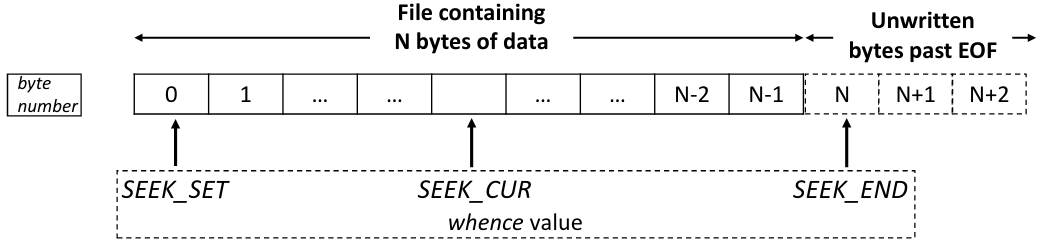
\includegraphics[width=0.5\textwidth]{lseek.png}
    \end{center}

    \subsection{close}

    \begin{lstlisting}[language=C]
        #include <unistd.h>

        //Returns 0 on success, or -1 on error
        int close(int fd);
    \end{lstlisting}
    Tutti i file descriptor vengono chiusi quando un processo 
    termina, ma è buona prassi chiudere sempre. La chiusura 
    \textbf{non} elimina il file. 

    \subsection{unlink}

    \begin{lstlisting}[language=C]
        #include <unistd.h>

        //Returns 0 on success, or -1 on error
        it unlink(const char *pathname);
    \end{lstlisting}
    Prende in input il nome del file, perché il file descriptor
    può anche essere chiuso, se il file non ha altri symbolic 
    link, viene rimosso.
    \begin{description}
        \item[Symbolic link:] il collegamento su desktop, oppure il file è aperto da altri processi. 
    \end{description}
    \verb|unlink| \textbf{non} può rimuovere directory.

    \subsection{stat, lstat, fstat}

    \begin{lstlisting}[language=C]
        #include <sys/stat.h>

        //Returns 0 on success, or -1 on error
        int stat(const char *pathname, struct stat *statbuf);
        int lstat(const char *pathname, struct stat *statbuf);
        int fstat(int fd, struct stat *statbuf);
    \end{lstlisting}
    In caso di succeso la \verb|struct stat| viene popolata da 
    varie informazioni. La differenza tra queste system call 
    sono: 
    \begin{itemize}
        \item \verb|stat| ritorna informazioni relative a un file tramite il nome o path;
        \item \verb|lstat| tramite symbolic link;
        \item \verb|fstat| utilizza il file descriptor;
    \end{itemize}
    
    \subsection{Mode}

    Si tratta di una bit mask, presente anche nella \verb|struct stat|
    , che ci permette di definire i permessi dei file. 
    Lunga 16 bit, i primi 9 sono per other, group e user, 
    rispettivamente 3 a testa. Possiamo usarla per avere 
    informazioni sulla tipologia del file. Esempio:
    \begin{lstlisting}[language=C]
        char pathname[] = "/tmp/file.txt";
        struct stat statbuf;
        //Getting the attribute of /tmp/file.txt
        if(stat(pathname, &statbuf) == -1)
            errExit("stat");

        //Checking if /tmp/file.txt is a regular file
        if((statbuf.st_mode & S_IFMT) == S_IFREG)
            prinf("regular file!\n);

        //Equivalently, checking if /tmp/file.txt is a 
        //regular file by S_ISREG macro
        if(S_ISREG(statbuf.st_mode))
            printf("regular file!\n");
    \end{lstlisting}
    \begin{center}
        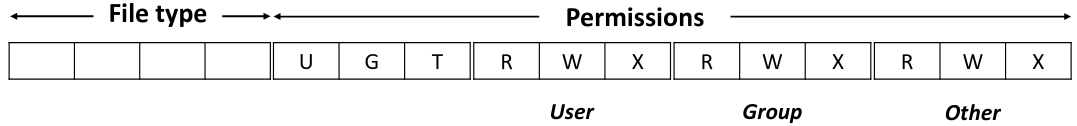
\includegraphics[width=0.5\textwidth]{st_mode.png}
    \end{center}
    I bit oltre i 9 dedicati a other, group e user hanno 
    i seguenti significati:
    \begin{itemize}
        \item U identifica se l'utente che sta eseguendo quell'eseguibile è lo stesso utente proprietario dell'eseguibile;
        \item G verifica se il gruppo che sta eseguendo è il gruppo proprietario;
        \item T è lo sticky bit, funziona come un bit che non ci permette di cancellare quel file;
    \end{itemize}
    File e directory sono la stessa cosa, per modificare i permessi 
    di una directory si usano le stesse mode dei file.

    \subsection{access}

    Controlla l'accessibilità di un file relativamento 
    al nostro user id e group id.
    \begin{lstlisting}[language=C]
        #include <unistd.h>

        //Returns 0 if all permissions are granted, otherwise -1
        int access(const char *pathname, int mode)
    \end{lstlisting}
    Le possibili mode che si possono usare insieme 
    a questa system call sono queste:
    \begin{center}
        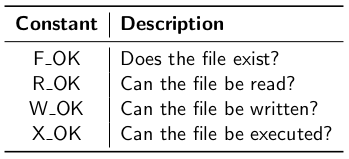
\includegraphics[width=0.5\textwidth]{access.png}
    \end{center}

    \subsection{chmod e fchmod}

    Permettono di cambiare i permessi di un file prendendo
    in input il pathname o il file descriptor più le eventuali
    mode di interesse.
    \begin{lstlisting}[language=C]
        //All return 0 on success, or -1 on error
        #include <sys/stat.h>

        int chmod(const char *pathname, mode_t mode);

        #define _BSD_SOURCE
        #include <sys/stat.h>

        int fchmod(int fd, mode_t mode);
    \end{lstlisting}

    \section{Directory}

    \subsection{mkdir}

    Prende in input il pathname della directory e 
    una mode.
    \begin{lstlisting}[language=C]
        #include <sys/stat.h>

        //Returns 0 on success, or -1 on error.
        int mkdir(const char *pathname, mode_t mode);
    \end{lstlisting}
    I parametri mode sono gli stessi della \verb|open|,
    se la directory esistesse già, il valore di ritorno sarà 
    sempre -1, ma la variabile \verb|errno| conterrà 
    il messaggio \verb|EEXIST|, a indicare che tale 
    directory è già presente.

    \subsection{rmdir}

    \begin{lstlisting}[language=C]
        #include <unistd.h>

        //Returns 0 on success, or -1 on error.
        int rmdir(const char *pathname);
    \end{lstlisting}
    Se esiste anche un solo file all'interno dello directory
    tale system call tornerà -1 di errore, per avere successso
    deve essere completamente vuota.

    \subsection{opendir, closedir e readdir}

    \begin{lstlisting}[language=C]
        #include <sys/types.h>
        #include <dirent.h>

        //Returns directory stream handler, or NULL on error.
        DIR *opendir(const char *dirpath);

        //Returns 0 on success, or -1 on error
        int closedir(DIR *dirp);
    \end{lstlisting}
    Una volta aperta una directory per leggerla si userà
    \begin{lstlisting}[language=C]
        #include <sys/types.h>
        #include <dirent.h>

        //Returns pointer to an allocated structure describing the
        //next directory entry or NULL on end-of-directory or error
        struct dirent *readdir(DIR *dirp);
    \end{lstlisting}
    La struttura di riferimento per la \verb|readdir|:
    \begin{center}
        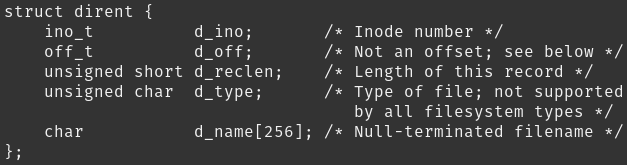
\includegraphics[width=0.5\textwidth]{dirent.png}
    \end{center}
    Tramite il \verb|d_type| possiamo ottenere delle informazioni
    sul tipo di file che stiamo scorrendo:
    \begin{center}
        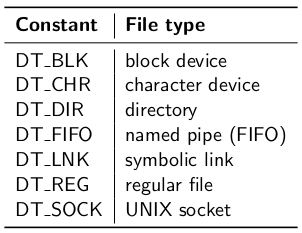
\includegraphics[width=0.5\textwidth]{d_type.png}
    \end{center}
    Esempio d'uso:
    \begin{lstlisting}[language=C]
        DIR *dp = opendir("myDir");
        if(dp == NULL)
            return -1;
        
        errno = 0;
        struct dirent *dentry;
        //Iterate until NULL is returned as a result
        while((dentry = readdir(dp)) != NULL){
            if(dentry->d_type == DT_REG)
                printf("Regular file: %s\n", dentry->d_name);
            errno = 0;
        }
        //NULL is returned on error, and when the end-of-directory is reached!
        if(errno != 0)
        printf("Error while reading dir.\n");
        closedir(dp);
    \end{lstlisting}


     


    
    








\end{document}